%*******************************************************************************
%*********************************** First Chapter *****************************
%*******************************************************************************

\chapter{Introduction}  %Title of the First Chapter

\ifpdf
    \graphicspath{{Chapter1/Figs/Raster/}{Chapter1/Figs/PDF/}{Chapter1/Figs/}}
\else
    \graphicspath{{Chapter1/Figs/Vector/}{Chapter1/Figs/}{Chapter1/Figs/PDF/}}
\fi


%********************************** %First Section  **************************************
\section{Research Background and Significance} %Section - 1.1
%人工智能的技术研究和商业化应用部署在近年来的发展显示了一种加速的趋势。各种基于人工智能和大数据分析相关算法的部署上线在加速企业、组织数字化,改善产业链结构和提高信息利用效率方面发挥了积极作用。教育行业作为传统的服务行业,也存在相当大的智能化革命的空间。在传统教育模式中,学生群体往往被分为班级这种基础教育单元。因而在一个班级中,所有的教学活动的粒度与班级的大小相当,这导致学生所学习的内容与其需求不完全匹配。也即,学生已经掌握的知识点过度练习或者未掌握的知识点缺乏练习。这造成了学生出现厌学、焦虑等状况,对其学习效率和学习效果造成了较大影响。另一方面,对于教师而言,普遍性的个体知识状态精细监测和评估需要巨大的工作量,因此教师往往只关注一部分学生,导致多数学生的学习情况被忽略。这对于学生的学习积极性和学习状况具有较大的影响。

The development of technological research and commercial application deployment of artificial intelligence has shown an accelerating trend in recent years. The deployment of various algorithms related to AI and big data analytics based on artificial intelligence plays a positive role in accelerating enterprises and organizations' digitization, improving industry chains' structure, and increasing information utilization efficiency. As a traditional service industry, the education industry also has considerable prospects for an intelligent revolution. In traditional education models, student groups are often divided into basic education units like classes. Therefore, in a class, the granularity of all teaching activities is equivalent to the class size, which leads to the fact that the content of students' learning does not entirely match their needs. The knowledge points that the students have mastered are over-practice, or the knowledge points that the students have not mastered lack practice, which has caused students to be tired of learning, anxiety, and other conditions, significantly impacting their learning efficiency and learning effect. On the other hand, for teachers, generalized detailed monitoring and evaluation of individual knowledge status require a considerable workload, so teachers often only pay attention to a part of the students, leading to the neglect of most students' learning situation, which has a more significant impact on students' learning enthusiasm and learning conditions.

%近年来,中国发布了一系列促进人工智能在教育领域的应用的政策。通过人工智能技术来进行学生的学习情况监测和追踪,可以解放教师的劳动力,还可以解决传统人工教育中难以解决的问题,从而大大改善教育质量和效率,实现智慧教育。在智慧教育中,自适应学习是一个已经实践验证过的模型,它已经拥有了许多商业化部署的成功案例。相当多的在线教育平台已经部署了不同领域的自适应学习教育系统服务。它运用数据分析、机器学习和自动化等技术,通过分析学生的学习行为数据,自动地对学生进行知识状态的评估和追踪。此外,该系统结合学生的潜能、擅长领域等等个性化信息,向学生提供学习路径规划和学习资源推荐服务。它在降低教师工作压力的同时,能够提升教师的教学质量,也能够有效地帮助学生提升学习的效率。习题推荐系统是一个自适应学习的实现,它包括学习者知识掌握熟练度建模和习题推荐两个部分。知识掌握熟练度建模的一般模式为,输入学习者的学习交互记录例如做题记录、测验记录等语义记录,捕获学习者的学习特征,实现对于其知识掌握熟练度的动态追踪。习题推荐部分则通过分析学习者的知识掌握熟练度模型,推荐与学习者的知识掌握相对薄弱的部分最相关的习题。

In recent years, China has released a series of policies to promote artificial intelligence in education. AI technology for student learning monitoring and tracking can free up teachers' labor and solve problems that are difficult to solve in traditional manual education, thus significantly improving the quality and efficiency of education and realizing smart education. In smart education, adaptive learning is a model that has been proven in practice, and it already has many successful cases of commercial deployment~\cite{chen2018recommendation}. A considerable number of online education platforms have deployed adaptive learning education system services in different domains. It uses data analytics, machine learning, and automation to automatically assess and track students' knowledge status by analyzing their learning behavior data. Besides, the system provides students with learning path planning and learning resource recommendation services by combining personalized information such as students' potential and areas of expertise~\cite{soltani2019adaptive}. It can improve teachers' teaching quality while reducing teachers' work pressure and effectively improve their learning efficiency. The exercise recommendation system implements an adaptive learning model, including learner knowledge mastery proficiency modeling and exercise recommendation. The general model of knowledge mastery modeling is to input the semantic records of learners' learning interactions such as question records, quiz records to capture learners' learning characteristics and achieve the dynamic tracking of their knowledge mastery proficiency. The exercise recommendation part analyzes the learners' knowledge mastery proficiency model and recommends exercises relevant to the learners' relatively weak knowledge mastery.

%高中数学学科是高中阶段相对较难的一门科目。目前,在高中数学学科中,知识点繁杂而且具有紧密的内在联系,对应的习题库也庞大而混乱。导致许多学生不知道如何去合理评估自己的知识掌握度从而有针对性地练习,导致``题海战术''的出现。这对于学生的学习兴趣和自信心有负面的影响。本文把高中数学学科作为研究背景,目的是提出一种实时追踪学生数学知识掌握情况,并依照学生的知识状态进行习题推荐的系统。该系统分为三个部分,第一个部分对习题进行知识点标注,作为习题推荐系统的数据准备部分,第二部分是核心的知识追踪模型,它通过输入学生的做习题记录来追踪知识熟练度状态,第三部分是系统的功能部分,它通过知识追踪模型输出的学生知识熟练度针对性地推荐习题。该系统可以有效地实现自适应学习的目标。

High school mathematics is a relatively tricky subject at the high school level. In high school mathematics, the knowledge points are complicated and closely interconnected, and the corresponding library of exercises is extensive and confusing. As a result, many students do not know how to reasonably assess their knowledge and practice in a targeted manner, leading to the emergence of ``excessive practicing tactics'', which hurts students' interest in learning and self-confidence. The purpose of this thesis is to propose a system for tracking students' knowledge of mathematics in real-time and recommending exercises according to their knowledge status. The system is divided into three parts: the first part is the knowledge labeling of the exercises as the data preparation part of the exercise recommendation system, the second part is the core knowledge tracing model, which tracks the knowledge proficiency status by inputting students' records of doing exercises, and the third part is the functional part of the system, which recommends exercises targeted by students' knowledge proficiency output from the knowledge tracing model. The system can effectively achieve the goal of adaptive learning.

%********************************** %Second Section  *************************************
\section{Related Works and Theories}
%本文的研究课题为高中数学习题推荐系统,

%如wang等人提出结合神经网络的认知诊断模型NeuralCD,在预测精度和可解释性上均有所提升。一种流行的方法是是通过认知诊断的方式来对学生的知识掌握状态进行评估,然后基于学生的知识状态来进行对应的习题推荐。

%第一个部分为基于图神经网络和自然语言处理的习题知识点标注,第二个部分为基于图注意力网络与Transformer的知识追踪模型,第三个部分为基于协同过滤和神经网络的习题推荐模块, 的知识跟踪与推荐系统等。因而本文涉及的技术包括高中数学图神经网络,自然语言处理,多标签分类,推荐系统等研究课题, 接下来,本节将回顾这些技术的研究现状。
\subsection{Related Works}
This thesis's research topic is a recommendation system for high school mathematics exercises, the core of which is to find the underlying factors that influence students' performance in answering questions. Some basic theoretical research and related experimental analysis and application deployments have emerged. Among them, cognitive diagnosis is a classical and effective method used to analyze students' learning performance. For example, Huang et al.~\cite{huang2017hcdm} applied multilevel structure into higher-order latent features to extend the original model into a multilevel higher-order cognitive diagnostic model; Ma et al. proposed a cognitive diagnostic model that applies multiple strategies to adapt to the strategic heterogeneity of different students~\cite{Ma2019MCDM}; and Wang et al.~proposed NeuralCD~\cite{wang2020neural}, a cognitive diagnostic model combined with neural networks, which has improved in both prediction accuracy and interpretability. Furthermore, some researchers have modeled the exercise recommendation problem as learning path recommendation and cognitive modeling, such as the CSEAL model proposed by Liu et al.~\cite{CSEALliu2019}, which incorporates Markov decision processes into student learning path planning, and a framework based on multidimensional knowledge graph proposed by Shi et al.~\cite{SHI2020105618} In addition, researchers have also tried to use a large amount of student interaction data from online education systems to mine students' learning status and use it for interactive exercise recommendations. Huang et al. proposed the DRE framework for recommending exercises to students with the greatest knowledge gain~\cite{DRE2019Huang}, which can also refer to student feedback to optimize its strategy, implementing the adaptive recommendation. At the application level, Choi et al. designed the Rocket system for student knowledge state visualization and improved the interpretability of exercise recommendations~\cite{choi2020choose}. 

When referring to knowledge tracing-based exercise recommendations, there emerged lots of related research recently. Cai et al. proposed a knowledge tracing to track the variance of knowledge proficiency of students to perform exercise recommendation~\cite{9064104}. Furthermore, Zhao et al. incorporated the user's auxiliary features into the knowledge tracking model and improved the interpretability of the model with the user's learning attributes~\cite{10.1145/3386527.3406739}. At the application level, Trifa et al. propose an intelligent agent system that incorporates knowledge tracking techniques for analyzing students' knowledge levels~\cite{trifa2019knowledge}. This system can be applied in an online learning platform and can output a view of the student's knowledge status.

The above studies all perform adaptive exercise recommendations based on students' knowledge state assessment, but none of them take into account the complexity of knowledge networks and the intrinsic connection of students' mastered knowledge points. In this thesis, this is improved by using knowledge tracking techniques in tracking students' knowledge states as well as recommending exercises. Thus, the theories and techniques related to this thesis include high school mathematics subjects, graph neural networks, natural language processing, multi-label classification, recommendation systems, and other research topics. Next, the current research status on these techniques and theories will be reviewed.

\subsection{High School Mathematics}
%无论在基础教育还是科学研究中,数学都是一门必要的的学科。数学是一门专门研究数量与空间形式之间关系的科学,其符号系统更加完整,公式结构清晰独特,文字和图像等语言表达方式也更加生动直观。在数学学科中,知识结构和认知结构的建立对于该学科的学习起着相当重要的作用。``认知结构''表示在人大脑当中陈述性知识的组织形式,而经过学习内化后的认知结构通过网络结构或图形展示出来的就是知识结构~\cite{tanujaya2017relationship}。学习者所需要学习的知识内容大多来源于前人在实践活动中的经验总结,其学习的过程就是对这些归纳好的知识进行认知学习,并不断对知识的结构进行消化、调整、重组,从而构建更为完善和适合自己的知识结构的过程,也是一个与创新思维结合的过程。在数学学科中,知识的掌握往往来自于实践,例如习题练习、证明推导等等。数学学科作为中学阶段的主要科目,具有高度抽象性、严密逻辑性与广泛应用性等特点。该学科知识体系是利用众多的抽象性知识概念建立起来的,并借助对这些概念知识进行学习与思维拓展,形成新的抽象性概念知识。此外,数学逻辑性十分严密,因为数学学科当中得出的任何结论,都需要经过严密的逻辑推理与严格的证明才能被认为是合理的。它是我们参与社会实践活动或科学研究的重要手段和工具,在各行各业以及社会的各个领域当中都离不开对数学的学习。数学知识点之间也具有内在关联性,因而它们可以在具体学习过程中根据特定的逻辑顺序进行安排和学习。这些内在关联关系可以分为同义关系、前驱关系、后继关系、包含关系、兄弟关系、对立关系等几种。通过对知识点进行分析,可以建立知识点关联网络,便于进行后续的知识状态追踪。


Mathematics is an essential subject in both primary education and scientific research. Mathematics is a science devoted to studying relationships between quantities and spatial forms, with a complete system of symbols, a clear and unique structure of formulas, and more vivid and intuitive verbal expressions such as words and images. In mathematics, the establishment of knowledge structure and cognitive structure plays a considerable role in learning the subject. The ``cognitive structure'' denotes the organization of declarative knowledge among the human brain, while the cognitive structure internalized through learning and displayed through network structures or graphics is the knowledge structure~\cite{tanujaya2017relationship}—most of the knowledge contents that learners need to learn come from the experience summaries in practical activities. The process of their learning is the cognitive learning of this summarized knowledge as well as constantly digesting, adjusting and reorganizing mastered knowledge. It is for building a more perfect and suitable knowledge structure, which is also a process of combining with innovative thinking. In mathematics, knowledge mastery often comes from practice, such as exercises, proofs, and derivations. As a primary subject at the secondary level, mathematics is characterized by a high degree of abstraction, rigorous logic, and extensive applications. The body of knowledge in this subject is built up using many abstract concepts, and new abstract concepts are formed by learning and expanding on these concepts. Also, mathematics is logical because any conclusion reached in mathematics requires rigorous logical reasoning and strict proof before it can be considered reasonable. It is an essential tool for social practice or scientific research, and the study of mathematics is indispensable in all walks of life and all areas of society. Mathematical knowledge is also intrinsically related to each other to be arranged and learned in a specific logical progression in the specific learning process. These intrinsic relationships can be classified as synonymous, antecedent, successor, inclusion, brotherhood, opposition, and so on. A network of knowledge point associations can be established to facilitate subsequent knowledge mastery status tracking by analyzing the knowledge points.

\subsection{Graph Neural Network}
%近年来,神经网络模型的高速发展推动了机器学习相关的研究,各种针对各类应用环境和任务的神经网络范式被设计出来,例如广泛应用于模式和特征识别领域的卷积神经网络范式(CNNs)以及应用于序列化数据学习的循环神经网络范式(RNNs)。传统神经网络对于欧几里得空间中的数据例如语言、序列、图片等具有较好的计算和处理能力,但对于非欧几里得空间例如知识网络则具有一定的局限性。本文中的研究对象为学科知识,知识点之间形成一个网状的关联关系,因此用传统的神经网络模型处理无法完全表征知识点间的复杂关系,以图来学习知识点网络则更加匹配。每个知识点或者习题可以作为图的节点,节点之间的边则代表知识点或习题之间的关联关系。因此本文引入了图神经网络来捕捉知识点和习题之间的关联性,可以在更高的维度对数据进行合理抽象,取得较好的效果。

%目前对于图结构,可以进行的机器学习任务可以粗略分为以下几种:
%(1)图节点分类任务:对于一个每个节点都有对应的特征的图,且部分节点的类别已知,可以设计分类任务针对未知节点进行分类。(2)图边结构预测任务:对于一个部分节点之间的边的关系已知的图,根据已有的信息来挖掘位置的边结构和关系,这类任务就是对边的预测任务,也就是对节点和节点之间关系的预测。(3)图的分类:对于整个图来说,我们也可以对图分类,图分类又称为图的同构问题,这往往通过聚合图的节点特征然后进行分类来实现。

In recent years, the rapid development of neural network models has driven research related to machine learning, and various neural network paradigms have been designed for various application environments and tasks. For example, there appear convolutional neural networks (CNNs), which are widely used in pattern and feature recognition, and recurrent neural networks (RNNs), which are applied to serialized data learning. Traditional neural networks have good computational and processing capabilities for data in Euclidean space such as language, sequences, and images, but have limitations for non-Euclidean space such as knowledge networks. In this thesis, the study object is mathematical subject knowledge, and the knowledge points form a net-like correlation between them. Therefore, the complex relationship between knowledge points cannot be fully characterized by traditional neural network model processing, and it is more compatible with the natural paradigm to learn the knowledge point network by the graph. Each knowledge point or exercise can be treated as a node of a graph, and the edges between nodes represent the association between knowledge points or exercises. Therefore, this thesis introduces a graph neural network to capture the correlation between knowledge points and exercises, which can reasonably abstract the data in a higher dimension and achieve better results.

At present, for the graph structure, the machine learning tasks that can be performed can be roughly divided into the following types:
\begin{enumerate}
    \item Graph node classification task: For a graph in which each node has a corresponding feature, and the categories of some nodes are known, a classification task can be designed to classify unknown nodes.
    \item Graph edge structure prediction task: For a graph where the edge relationship between some nodes is known, the edge structure and relationship of the location are mined based on the existing information. This type of task is the edge prediction task: Prediction of the relationship between nodes and nodes.
    \item Graph classification: graph classification is also called the graph isomorphism problem, which is often achieved by aggregating the node characteristics of the graph and then classifying it.
\end{enumerate}

%图神经网络在2009年由Franco等人提出,该模型基于不动点理论,目的是获得每个节点的隐藏状态。但当堆叠次数过多时,该状态收敛容易过于平滑而导致难以学习图的特征信息。图神经网络一般以迭代的方式来对节点进行数据传递计算,以此学习目标节点表示。图神经网络的概念和应用经历了不断的发展,接连有新的图神经网络模型被提出来。近年来随着GPU等并行计算设备算力的提高,使得许多过于由于计算能力限制而无法应用的图神经网络模型有了实践应用的可能性。在本文中,主要用到了图卷积神经网络(GCN)和图注意力神经网络(GAT)等。GCN是Kipf于2016年提出的用于半监督分类的模型~\cite{kipf2017semi},GCN的计算是基于层级结构,每一层都是上一层的特征抽取的结果,从节点层面,节点之间互相传播隐藏状态。最终GCN输出经过多层抽象的结果,在对节点特征信息学习和图结构信息的学习方面,在大多数公开节点分类或边预测相关的数据集上GCN几乎均取得了State of the Art(SOTA)的性能表现。GAT是由Veličković等人在2018年提出~\cite{veličković2018graph},该网络在传播过程引入自注意力机制,每个节点的隐藏状态通过注意其邻居节点来计算。该网络采用了局部网络的设计结构,因此在计算过程中只计算相邻节点,降低了计算负载。

The graph neural network model is based on the theory of immobile points and aims to obtain the hidden state of each node~\cite{kim2019edge}. However, when there are too many stacks, the state convergence tends to be too smooth and challenging to learn the graph's feature information. Graph neural networks are generally applied iteratively to compute data transfer to nodes as one method to learn the target node representation. The concept and application of graph neural networks have undergone continuous development, and new graph neural network models have been proposed one after another. In recent years, the increase in computing power of parallel computing devices such as GPUs has made it possible to apply many graph neural network models that were too limited by computing power. In this thesis, a network structure similar to graph convolutional neural networks (GCN) is applied. GCN is a model proposed by Kipf in 2016 for semi-supervised classification~\cite{kipf2017semi}, and the computation of GCN is based on a hierarchical structure, where each layer is the result of feature extraction from the previous layer, from the node level, and the nodes propagate each other hiding the state. The final GCN output undergoes multiple layers of abstraction, and in terms of learning of node feature information and graph structure information, GCN achieves State of the Art (SOTA) performance on almost all of the datasets related to most public node classification or edge prediction. GAT was proposed by Veličković et al. in 2018~\cite{veli2018graph}. The network introduces a self-attentive mechanism in the propagation process, where the hidden state of each node is computed by paying attention to its neighboring nodes. The network uses a local network design structure so that only neighboring nodes are computed during the computation, reducing the computational load.

\subsection{Knowledge Tracing}
%知识跟踪(KT)是一项可根据学生过去的答题记录与结果对学生的知识掌握程度进行建模的技术,它是模拟学习者知识掌握情况的一个典型模型,目前已经发展成为智能辅导系统中对学习者知识掌握情况建模的主流方法。知识追踪的主要任务是根据学习者的的历史学习记录来分析学习者的知识掌握情况,从而自动跟踪学生的知识水平随时间的变化,以便能够准确地预测学生在未来学习中的表现并提供适当的学习辅导。 在此过程中,知识空间用于描述学生知识获取的水平。 在知识追踪的过程中,知识空间被建模为概念的集合,学生对概念集合的一部分的掌握构成了学生对知识的掌握。 一些教育研究人员认为,学生对一组特定的相关知识点的掌握会影响他们在练习中的表现,即学生已掌握的知识集与他们在练习上的外部表现密切相关。教师可以通过评估学生的知识状态来更好地了解学生知识掌握的薄弱之处,针对性地对教学方案进行调整。

%在知识追踪模型中,传统的方式是通过认知诊断的方式来实现,它是一种对学生进行知识点熟练度建模的算法。其中,Item response theory(IRT)~\cite{embretson2013item}基于一维连续模型对学习者进行建模,而DINA模型则基于一系列表示用户对习题相关知识掌握的向量来对学生进行知识状态建模~\cite{de2009dina}。除此之外,贝叶斯知识追踪(BKT)是一种应用较为广泛的基于概率图模型的知识追踪模型~\cite{yudelson2013individualized},它将学习者的知识状态建模为一组二进制变量,代表是否掌握知识点,该算法利用隐马尔可夫模型(HMM)来维护知识熟练度变量。但BKT的缺陷在于忽略了学生对于知识的遗忘特性和知识点之间的关联性。在2015年,深度知识追踪(DKT)被提出来~\cite{piech2015deep},它是首个将RNN模型应用于知识追踪任务的算法,该模型利用LSTM来追踪学生的知识熟练度随时间动态变化的过程,并学习出学生的知识掌握向量,利用该向量预测学生的做题表现。而2017年提出的Dynamic Key-Value Memory Networks for Knowledge Tracing(DKVMN)模型借用了记忆增强网络的思想,可以利用基础概念之间的关系,用一个键矩阵来存储学生对于知识概念的掌握水平,因此该模型可以显式地输出学生对于知识点的掌握成程度。该模型细化了习题与知识点之间的关系,在公开数据集上也取得了比DKT和BKT更优秀的表现。但是,这些模型都未将知识点的复杂关联性进行合适的建模,因此对于知识点关联复杂的习题,会出现预测性能下降的情况。而图神经网络作为一种适配非欧氏空间建模的模型,可以作为对知识点关系网建模的一种解决方案。在ICLR2019提出的Graph-based Knowledge tracing模型~\cite{nakagawa2019graph},利用图节点来对学生的回答的习题建模,考虑了做题对于知识状态以及相似习题的影响,在公开数据集的测试结果表名该模型的表现超过了DKVMN。

Knowledge tracing is a technology that models student knowledge acquisition based on past answer records and results. It is a classical model for modeling learner knowledge acquisition and has evolved into the mainstream approach for modeling learner knowledge acquisition in intelligent tutoring systems. The main task of knowledge tracing is to analyze learners' knowledge mastery based on their historical learning records and thus automatically track changes in students' knowledge levels over time in order to be able to accurately predict students' performance in future learning and provide appropriate learning tutoring. In this process, the knowledge space is used to describe the level of student knowledge acquisition. In the process of knowledge tracing, the knowledge space is modeled as a collection of concepts, and students' mastery of a portion of the collection of concepts constitutes students' mastery of knowledge. Some educational researchers argue that students' mastery of a specific set of related knowledge points affects their performance on exercises, i.e., the set of knowledge students have mastered closely related to their external performance. Teachers can assess students' knowledge status to understand better where their mastery is weak and target their instructional programs.s

In the knowledge tracing model, the traditional approach is implemented by cognitive diagnosis, an algorithm for modeling students' proficiency in knowledge points. Among them, Item response theory (IRT)~\cite{pliakos_integrating_2019} models learners based on a one-dimensional continuous model, while the DINA model models students' knowledge states based on a series of vectors that represent users' knowledge mastery related to the exercises~\cite{huang2020utilizing}. Besides, Bayesian knowledge tracing (BKT) is a more widely used knowledge tracing model based on probabilistic graphical modeling~\cite{yudelson2013individualized}, which models the learner's knowledge state as a set of binary variables representing whether the knowledge points are mastered or not, and the algorithm uses Hidden Markov Model (HMM) to maintain the knowledge proficiency variables. However, the drawback of BKT is that it ignores the forgetting property of students for knowledge and the correlation between knowledge points. In 2015, Deep Knowledge Tracing (DKT) was proposed~\cite{piech2015deep}, which is the first algorithm to apply RNN models to the knowledge tracing task, and the model uses LSTM to track the dynamic change of students' knowledge proficiency over time and learn the student's knowledge mastery vector, which is used to predict students' performance on questions.

Moreover, the Dynamic Key-Value Memory Networks (DKVMN) for knowledge tracing model proposed in 2017 borrows the idea of memory-enhanced networks, which can store students' mastery levels of knowledge concepts using a fundamental matrix by using the relationships between the underlying concepts, so the model can Explicitly output the student's mastery of the knowledge point. The model defines the relationship between exercises and knowledge points and achieves better performance than DKT and BKT on public datasets. However, these models do not appropriately model the complex correlation of knowledge points and degrade the prediction performance for exercises with complex knowledge point associations. In contrast, as a model adapted to model non-Euclidean spaces, a graph neural network can be a solution to model the relational network of knowledge points. The Graph-based knowledge tracing model proposed at ICLR2019~\cite{nakagawa2019graph}, which uses graph nodes to model student's responses to the exercises, considers the effect of doing questions on the knowledge state as well as similar exercises, and the test results in the public dataset tabulate the performance of this model over DKVMN.


\subsection{Recommendation System}
%在互联网发展早期,用户往往是通过搜索取寻找感兴趣的内容,但随着互联网信息的海量增长,搜索合适的内容已经变得越来越困难,因此立足于向用户推送他们感兴趣的信息的推荐系统技术被开发出来。目前推荐系统已经在互联网上得到了广泛的应用,无论给服务提供方还是给用户都带来了巨大的收益。在教育领域,对于广大的学生来说,现有的习题库过于繁杂,因此学生在进行课外练习的过程中往往会产生信息迷航的现象。通过自行寻找习题进行练习的方式效率低且容易出现知识误区。因此一个基于学生的知识状态进行自适应习题推荐的系统是必要和重要的~\cite{tan2008learning}。

%推荐系统目前有几大类算法:协同过滤,基于内容的推荐模型等。协同过滤算法的核心思想是将用户分为基于相似兴趣的群体,依照这个原理来寻找与被推荐者兴趣相似的用户,将该群体感兴趣的内容推荐给用户。协同过滤算法综合相似用户对推荐项目的评价,形成一个用户对项目的兴趣预测模型。协同过滤是目前应用最为广泛和成功的推荐算法之一。协同过滤又可以进一步细分为两种:基于用户的模式和基于项目的模式~\cite{su2009survey}。其中,前者着重于寻找相似的用户,即推荐主体,然后通过相似推荐主体感兴趣的内容进行推荐,后者则着重于寻找相似的项目,即推荐项,通过通过计算项目相似度,筛选出最相似的推荐项目作为推荐结果。在协同过滤中,对相似度的计算是一个关键问题。目前已经有的相似度算法有Jaccard系数~\cite{leeJ2020accardcf}、余弦相似~\cite{wang2006unifying}、相关相似性~\cite{mclaughlin2004collaborative}等,协同过滤往往存在``冷启动''问题,即当相似用户或条目较少时,出现性能的较大退化。因此在推荐模型的起始阶段,可以采用随机推荐或者其他内容推荐方法。基于内容的推荐模型则根据用户的兴趣条目的特征进行兴趣模式挖掘,本质上是建立一个对项目的兴趣度计算模型,该方法不依赖于其他的用户,但该模型容易出现重复推荐的问题,因此需要额外的步骤进行去重操作~\cite{gopalan2014content}。

In the early days of the Internet, users often searched for the content of interest. However, with the massive growth of Internet information, it has become difficult to search for suitable content. Therefore, it is based on pushing users the information they are interested in. Recommendation system technology was developed. At present, the recommendation system has been widely used on the Internet, and it has brought considerable benefits to both service providers and users. In the field of education, for most students, the existing exercise database is too large, so students often experience information tragedy in the process of extracurricular exercises. The learning efficiency is relatively low. Therefore, a system for adaptive exercise recommendation based on students' knowledge status is necessary and important~\cite{huang2019exploring}.

There are several types of algorithms in recommendation systems: collaborative filtering, content-based recommendation models, and so on. The core idea of a collaborative filtering algorithm is to divide users into groups based on similar interests, and according to this principle, to find users with similar interests to the recommended person and recommend the content that the group is interested in the user. The collaborative filtering algorithm integrates similar users' evaluation of recommended items to form a prediction model of users' interest in the item. Collaborative filtering is one of the most widely used and successful recommendation algorithms. Collaborative filtering can be further subdivided into two types: user-based model and item-based model~\cite{Juan_2019}. The former focuses on finding similar users, i.e., recommendation subjects, and then recommending them through the content of interest to similar recommendation subjects. In contrast, the latter focuses on finding similar items, i.e., recommendation items, and filtering out the most similar recommendation items as recommendation results by calculating the item similarity. In collaborative filtering, the calculation of similarity is a key issue. There are already similarity algorithms such as Jaccard coefficient~\cite{leeJ2020accardcf}, cognitive similarity~\cite{cogsim2020}, Kullback-Leibler divergence based similarity~\cite{kldsim2019}, etc. Collaborative filtering often has a ``cold boot'' problem~\cite{fu2019collaborative}, i.e., when there are fewer similar users or entries, a large performance degradation occurs. Therefore, random recommendations or other content recommendation methods can be used in the recommendation model's starting phase. On the other hand, the content-based recommendation model performs interest pattern mining based on the characteristics of the user's interest entries, which essentially builds a model for calculating the degree of interest in an item, and the method does not depend on other users. However, the model is prone to the problem of duplicate recommendations and thus requires an additional step for de-duplication operations~\cite{gopalan2014content}.

%********************************** % Third Section  *************************************
\section{Research Objectives and Content}  %Section - 1.3
%本研究的目的是提出一种基于知识追踪的的高中习题推荐系统,该系统分为三个部分,第一个部分为习题知识点标注部分,该部分的目的是为众多未标注的习题进行知识点标签分类,该模型为一个多知识点标签分类问题,在本节需要对中文数学习题进行文本挖掘,建立知识点标注模型,并对模型进行性能测试。第二个部分,将标注知识点的习题用作知识追踪模型的输入,该部分通过图神经网络进行习题知识图嵌入表示学习,设计一个基于Trasnformer结构的知识追踪模型来对学生的知识掌握熟练度状态进行跟踪并预测下一道习题的正确概率,同时该模型输出隐藏知识状态向量,用在后面的推荐部分作为下一级输入。最后一个部分,设计基于召回-排序两个阶段的推荐模型,先对习题进行初步过滤,筛选出候选推荐习题,然后输入知识追踪模型预测答题正确概率,按照错误率越高优先级越高的排序规则输出一个最终的习题推荐列表。

The purpose of this study is to propose a high school exercise recommendation system based on knowledge tracing, which is divided into three parts: the first part is the exercise knowledge point labeling part. This section requires text mining of math exercises, building a knowledge point labeling model, and performance testing of the model. In the second part, the labeled knowledge point exercises are adopted as the input of the knowledge tracing model. It learns the knowledge graph embedding representation of the exercises through graph neural networks, designs a knowledge tracing model based on the DKVMN model to track the students' knowledge mastery proficiency state and predict the correct probability of the next exercise, and outputs the hidden knowledge state vector, which is used in the later recommendation section as the next level input. In the last part, a recommendation model based on two stages of matching and ranking is designed first to filter the exercises to filter the candidate recommended exercises, then apply the knowledge tracing model to predict the probability of correct answers, and output a final list of recommended exercises.

\section{Thesis Organization and Structure}
%本文的第一章是导论。 介绍了研究的研究背景,相关技术、理论的研究进展和综述。描述了本文的研究重点和目标,基于目前已有的模型进行需求分析,提出基于知识追踪习题推荐系统的解决方案并分为三个模块:习题知识点标注,知识跟踪和习题推荐。本文的第2章着重于习题知识点标注,在习题资源推荐系统中,需要对解析出习题的知识点,然后根据学生当前的知识掌握情况,针对性地推荐学生掌握不足的知识点相关习题。本章节的算法模型分为习题文本信息抽取和标签标注两个部分,在实验部分通过与若干baseline模型进行性能对比实验来验证模型的有效性。本文的第3章提出了一个基于图神经网络的知识追踪模型,该模型分为习题-知识点关系嵌入学习、知识状态编码和答题预测解码三个部分。文中先对设计思路和相关技术进行理论介绍,然后在实验部分通过在公开数据集上与基准模型进行对比,验证模型的有效性并评估模型性能。本文的第4章提出了一种基于召回和排序两个阶段的推荐系统模型,该模型的召回阶段,通过多路召回策略分别召回多个候选习题子集,然后经过加权排序融合为最终的候选习题集。在模型的排序阶段,将候选习题集中的习题作为知识追踪模型的输入,然后收集习题的正确概率,进行优先级排序从而获得推荐习题列表。本文的第5章提出了结论和对于模型各个部分的未来的改进方向。

%第三章提出了一种针对动态键值记忆网络(DKVMN)的改进模型。该模型继承了原始DKVMN模型的基于知识点权重计算习题和学生掌握相关度的思想,相对于原始的DKVMN模型有如下改进。第一个改进是尝试在模型中融入答题延迟、请求提示等学生答题特征,从而捕捉学生的个性化特征对于习题解答的影响。另外,原始DKVMN模型未考虑到相关知识点的相互影响,而是将知识点作为独立的记忆单元。针对这一点,模型的第二个改进点是将图神经网络的信息传播思想融入模型,在对模型进行知识点掌握熟练度进行修正的过程中,运用图网络相邻节点传播机制,对相关知识点重新调整熟练度变化,从而为模型增加了对于知识点间关系的表征能力。在实验阶段,在公开的数据集上与原始DKVMN模型和一些其他的基线模型进行多方面的对比。结果显示,模型的性能和可解释性相对于原始的DKVMN模型以及其他的基线模型有一定的提升

Chapter 1 of this thesis is an introduction. The study's research background, motivation, and review of related techniques and theories are introduced. Besides, the research focus and objectives of this thesis are described. Based on the currently available models for requirements analysis, a solution based on a knowledge tracing exercise recommendation system is proposed and divided into three modules: exercise knowledge point labeling, knowledge tracing, and exercise recommendation.

Chapter 2 of this thesis focuses on the knowledge point labeling to the exercises. In the exercise resource recommendation system, it is necessary to analyze the exercises' knowledge points and then recommend exercises in which the knowledge points students have insufficient mastery. The model is composed of two parts: exercise text information extraction and multi-label knowledge classifiers generator. In the experimental part, the model's effectiveness is verified by conducting performance comparison experiments with several baseline models.

Chapter 3 of this thesis proposed an improved knowledge tracing model for DKVMN, divided into parts such as student answering behavior characterization, exercise knowledge weight calculation, knowledge mastery calculation, and knowledge mastery modification. The thesis starts with a theoretical introduction of the design idea and related techniques and then verifies the model's validity and evaluates the model performance by comparing it with the baseline model on a public dataset in the experimental part.

Chapter 4 of this thesis proposed a recommendation system model consists of two phases: matching and ranking. In the matching phase of the model, multiple candidate exercise subsets are generated separately by a multiplex-matching algorithm and then merged into the weighted ranking candidate exercises' final set. In the model's ranking phase, the candidate set exercises are used as the input to the knowledge tracing model, and then the exercises that are predicted to be mistaken would be collected and prioritized to generate a list of recommended exercises.

Chapter 5 of this thesis presents the conclusions and future directions for improving each part of the model. The overview structure of the thesis is shown in \figurename{\ref{fig:ch1-ov}}.
\begin{figure}[htbp!]
    \centering
    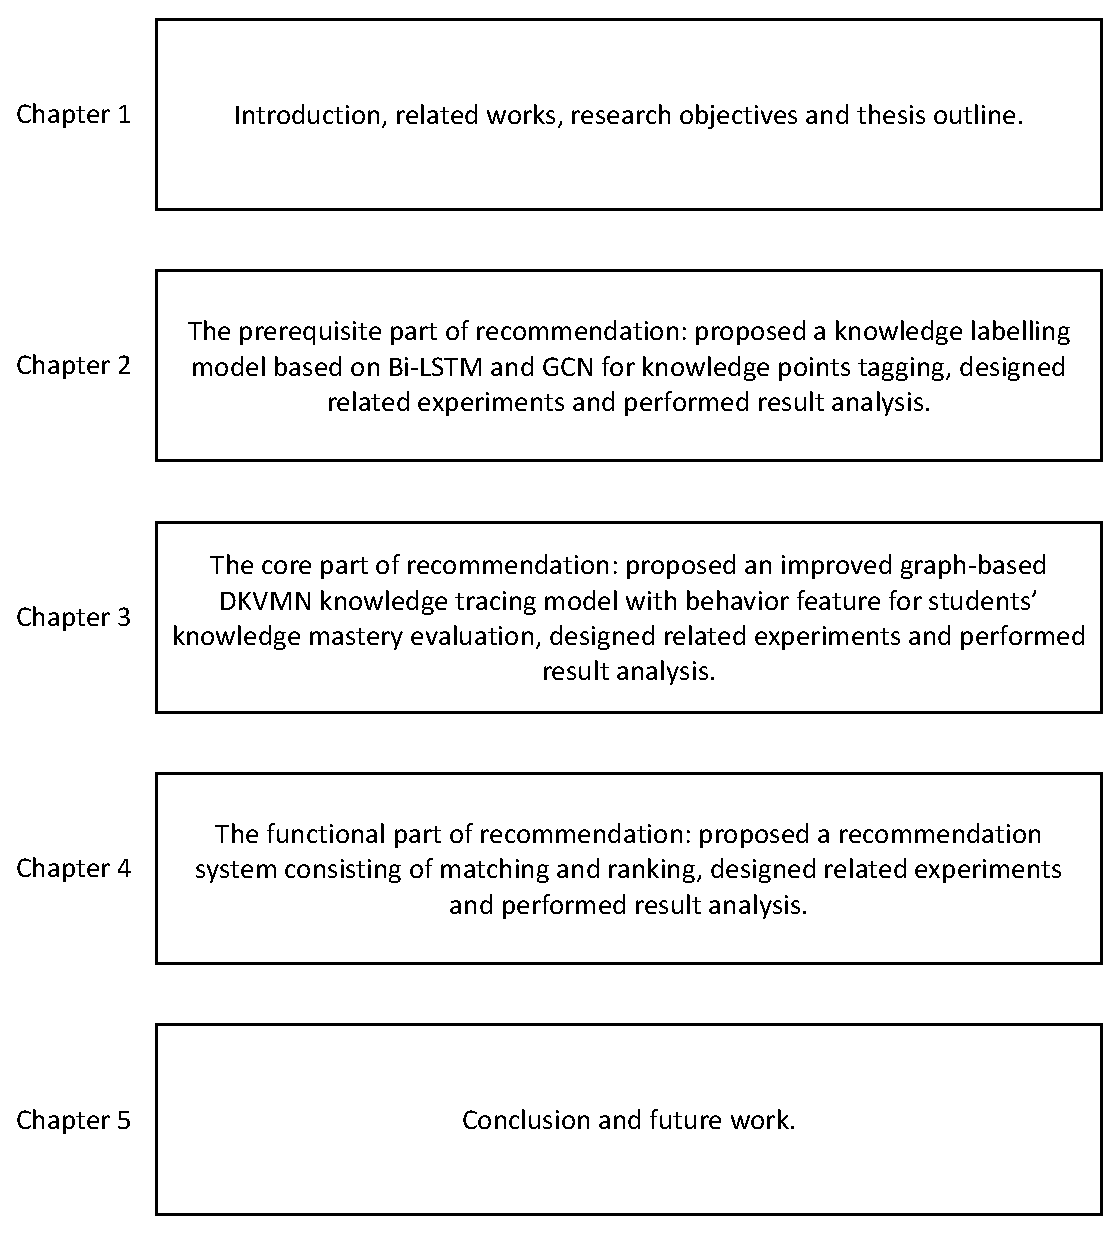
\includegraphics[width=1.0\textwidth]{ch1-ov.pdf}
    \caption{The structure of the thesis.}\label{fig:ch1-ov}
\end{figure}



% \nomenclature[z-DEM]{DEM}{Discrete Element Method}
% \nomenclature[z-FEM]{FEM}{Finite Element Method}
% \nomenclature[z-PFEM]{PFEM}{Particle Finite Element Method}
% \nomenclature[z-FVM]{FVM}{Finite Volume Method}
% \nomenclature[z-BEM]{BEM}{Boundary Element Method}
% \nomenclature[z-MPM]{MPM}{Material Point Method}
% \nomenclature[z-LBM]{LBM}{Lattice Boltzmann Method}
% \nomenclature[z-MRT]{MRT}{Multi-Relaxation
% 	Time}
% \nomenclature[z-RVE]{RVE}{Representative Elemental Volume}
% \nomenclature[z-GPU]{GPU}{Graphics Processing Unit}
% \nomenclature[z-SH]{SH}{Savage Hutter}
% \nomenclature[z-CFD]{CFD}{Computational Fluid Dynamics}
% \nomenclature[z-LES]{LES}{Large Eddy Simulation}
% \nomenclature[z-FLOP]{FLOP}{Floating Point Operations}
% \nomenclature[z-ALU]{ALU}{Arithmetic Logic Unit}
% \nomenclature[z-FPU]{FPU}{Floating Point Unit} 
% \nomenclature[z-SM]{SM}{Streaming Multiprocessors}
% \nomenclature[z-PCI]{PCI}{Peripheral Component Interconnect}
% \nomenclature[z-CK]{CK}{Carman - Kozeny}
% \nomenclature[z-CD]{CD}{Contact Dynamics}
% \nomenclature[z-DNS]{DNS}{Direct Numerical Simulation}
% \nomenclature[z-EFG]{EFG}{Element-Free Galerkin}
% \nomenclature[z-PIC]{PIC}{Particle-in-cell}
% \nomenclature[z-USF]{USF}{Update Stress First}
% \nomenclature[z-USL]{USL}{Update Stress Last}
% \nomenclature[s-crit]{crit}{Critical state}
% \nomenclature[z-DKT]{DKT}{Draft Kiss Tumble}
% \nomenclature[z-PPC]{PPC}{Particles per cell}
